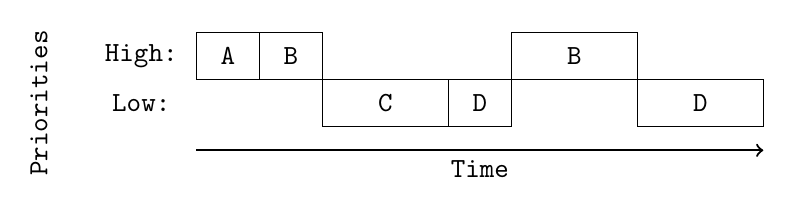
\begin{tikzpicture}[font=\ttfamily]

    % Style for general text nodes
    \tikzset{lbl/.style={inner sep=1pt, align=center}}

    % Define vertical coordinates for rows and labels
    \def\barheight{0.6} % Height of each bar
    \def\vtopprio{1.5}   % Vertical center of the top bar row
    \def\vsecprio{\vtopprio - \barheight} % Vertical center of the CM' bar row
    \def\ytimeline{\vsecprio - \barheight} % Vertical position of the minor frames timeline

    % Define standard tick positions
    \def\timeslice{0.8}

    % --- Bar Rows (drawn inside outlines) ---

    % Row 1: Top prio
    \draw (0, \vtopprio-\barheight/2) rectangle (\timeslice, \vtopprio+\barheight/2) 
      node[lbl, midway]{A};
    \draw (\timeslice, \vtopprio-\barheight/2) rectangle (\timeslice*2, \vtopprio+\barheight/2)
      node[lbl, midway]{B};

    % Row 2: Second prio
    \draw (\timeslice * 2, \vsecprio-\barheight/2) rectangle (\timeslice * 4, \vsecprio+\barheight/2)
      node[lbl, midway]{C};
    \draw (\timeslice * 4, \vsecprio-\barheight/2) rectangle (\timeslice*5, \vsecprio+\barheight/2)
      node[lbl, midway]{D};

    \draw (\timeslice*5, \vtopprio-\barheight/2) rectangle (\timeslice*7, \vtopprio+\barheight/2)
      node[lbl, midway]{B};

    \draw (\timeslice * 7, \vsecprio-\barheight/2) rectangle (\timeslice*9, \vsecprio+\barheight/2)
      node[lbl, midway]{D};

    % --- Left Vertical Label ---
    \node[lbl, rotate=90] at (-2.0, {\vsecprio}) {Priorities};
    \node[lbl] at (-0.7, {\vtopprio}) {High:};
    \node[lbl] at (-0.7, {\vsecprio}) {Low:};

    % Timeline axis with arrow and label
    \draw[thick, ->]
        (0, \ytimeline)
        -- node[below] {Time}
        (9*\timeslice, \ytimeline);
\end{tikzpicture}

